\begin{footnotesize}
	
	\node (ledger) at (0, 3) {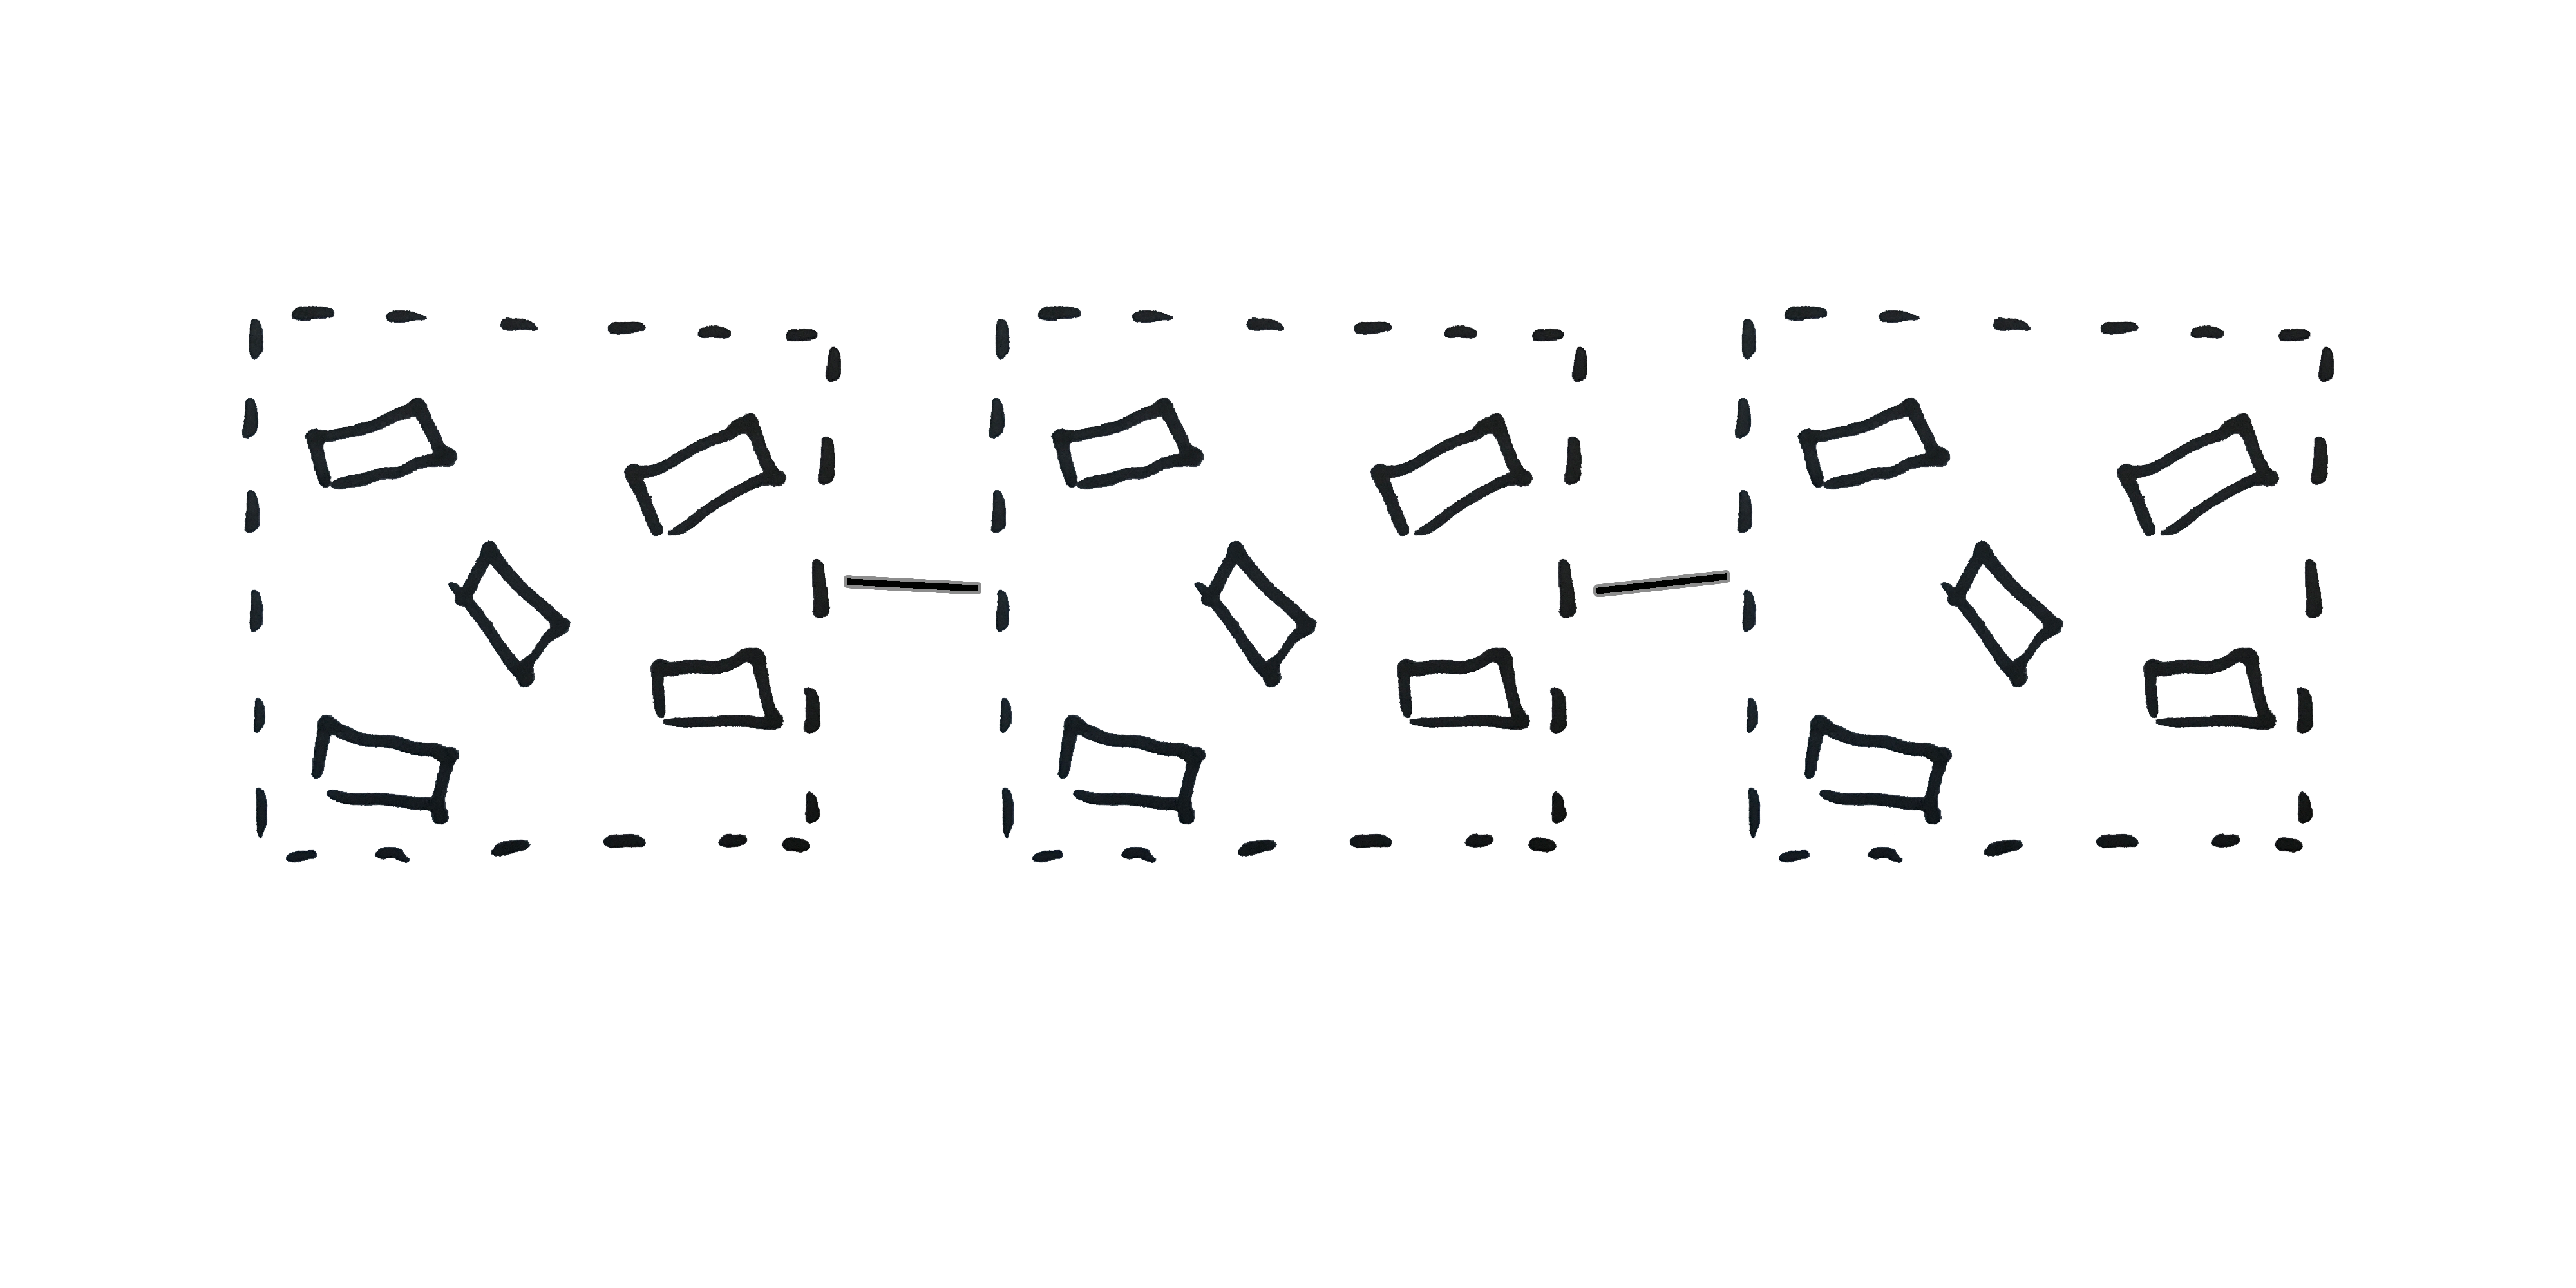
\includegraphics[height = 0.3\textheight, rotate = -90]{../assets/images/blocks_3}};
	\node (newblock) at (0, -1.8) {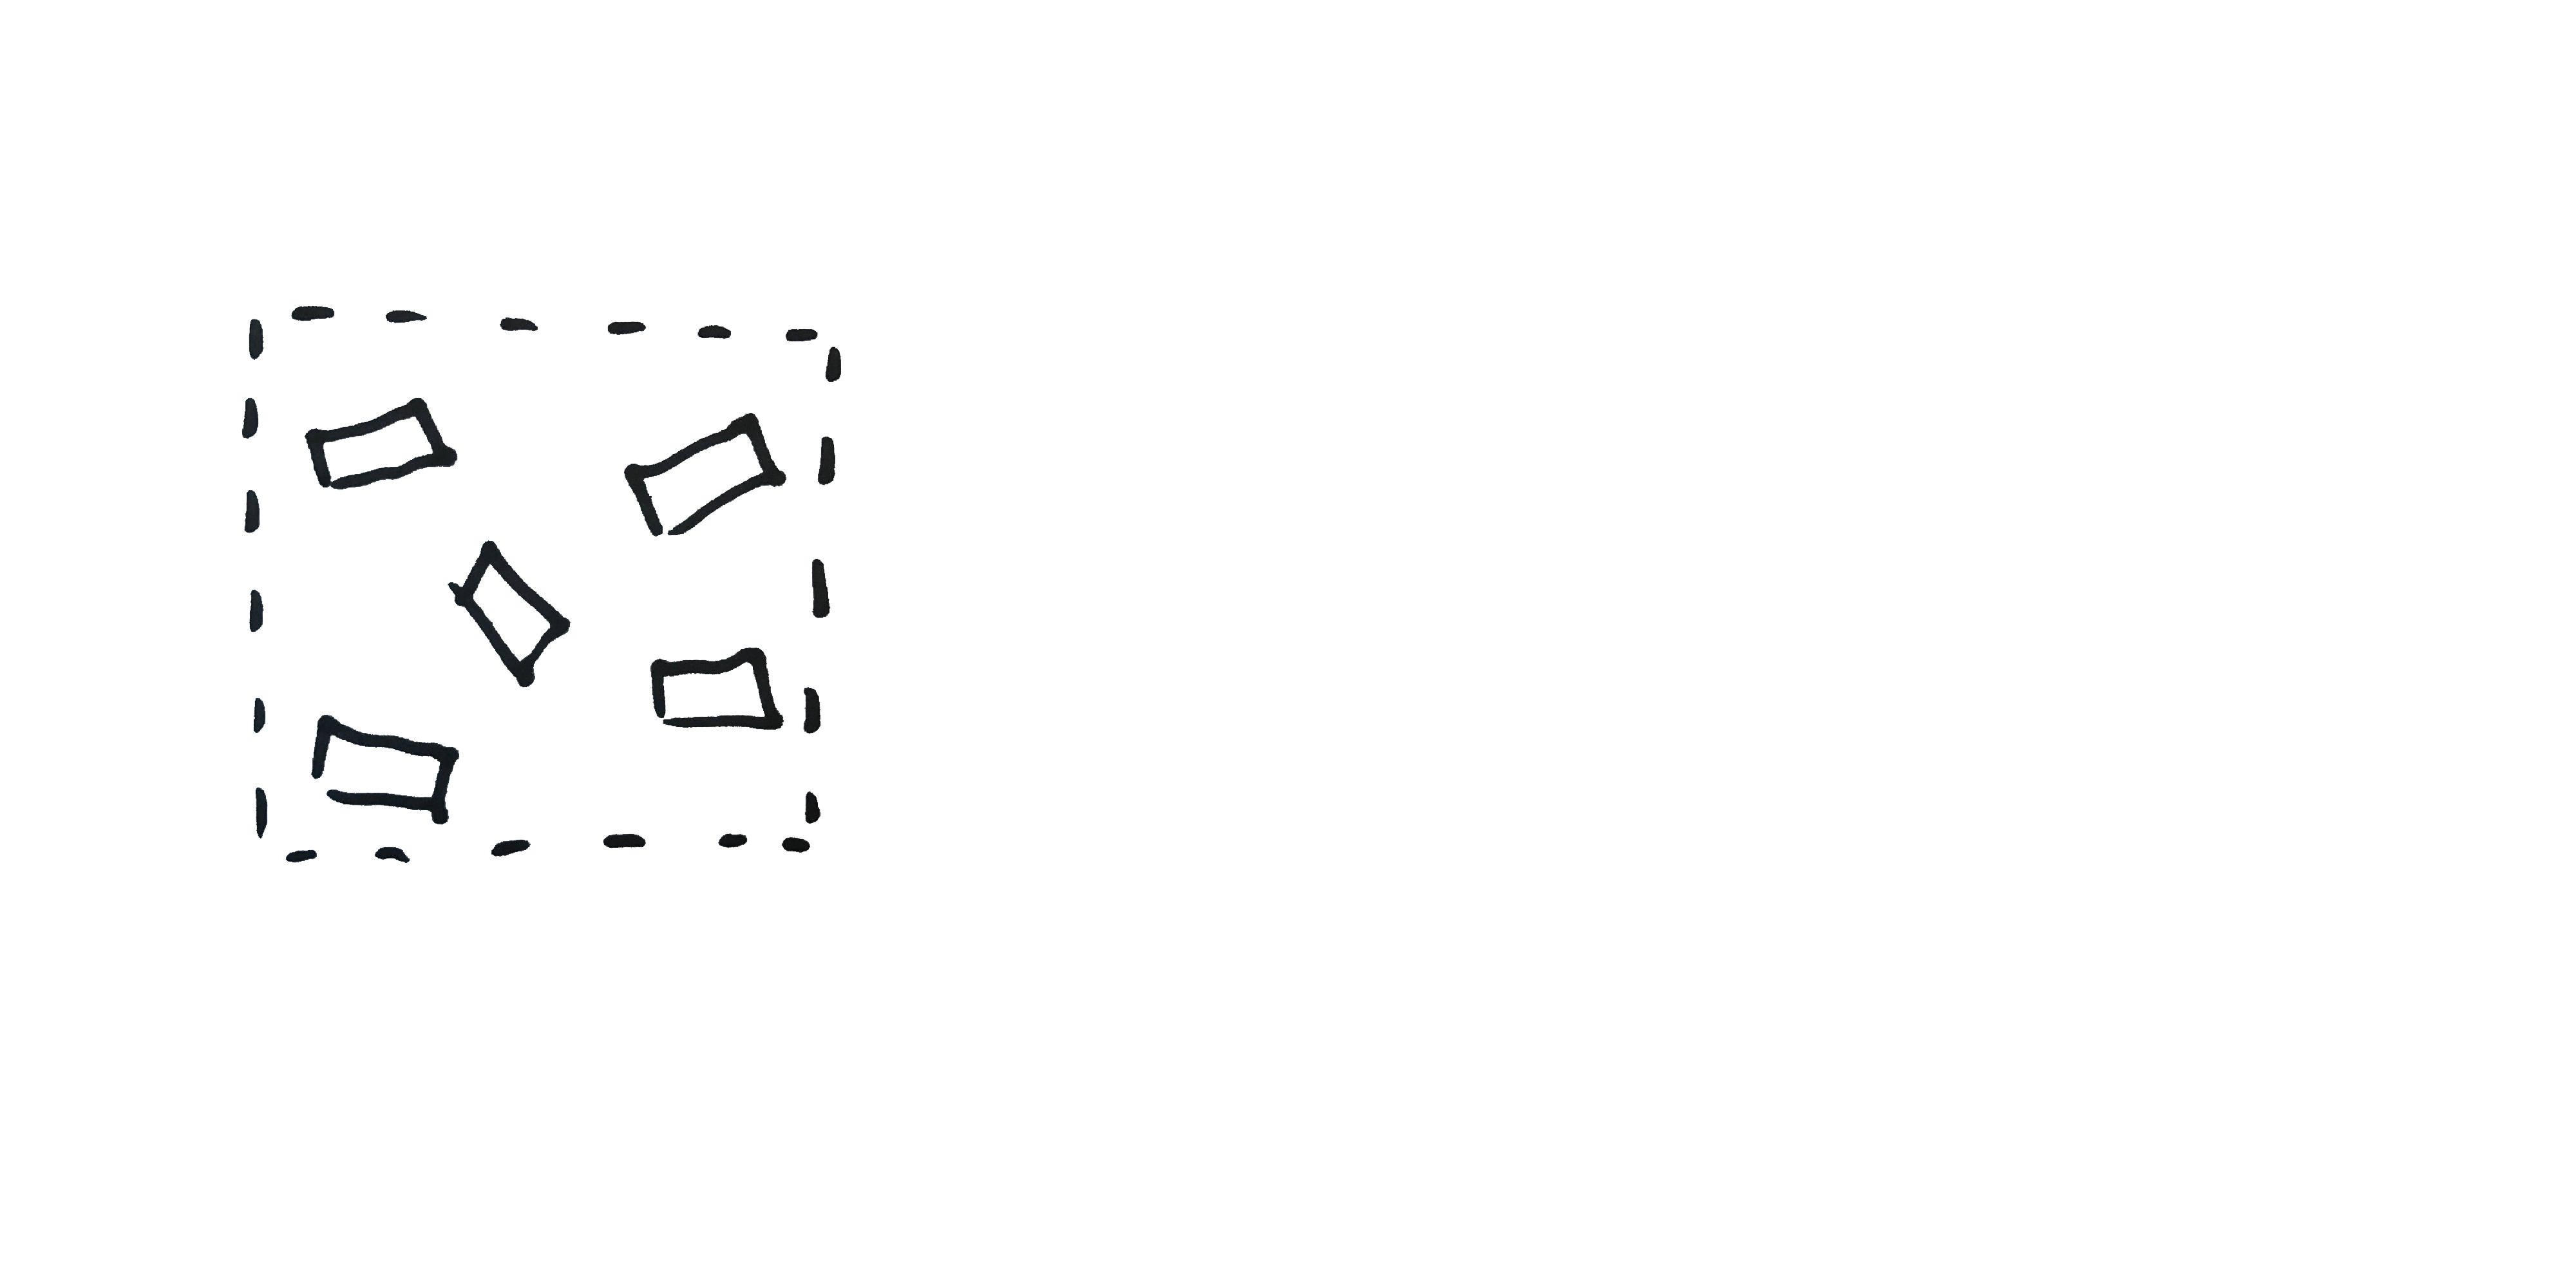
\includegraphics[height = 0.3\textheight, rotate = -90, decodearray={0.65 .8 0.84 .8 0.82 .8}]{../assets/images/block_1}};
	\draw[dashed, line width=0.35mm, color = highlight] (0.1, 0.8) -- (0.1, 0.4);
	\node (client) at (2, 2) {
\includegraphics[height = 0.2\textheight]{../assets/images/agents/handing_right}};
	\node (agent1) at (6, 4) {
\includegraphics[height = 0.2\textheight]{../assets/images/agents/reaching_left}};
	\node (agent2) at (6, 0) {
\includegraphics[height = 0.2\textheight]{../assets/images/agents/reaching_left}};
	\node (block) at (client) {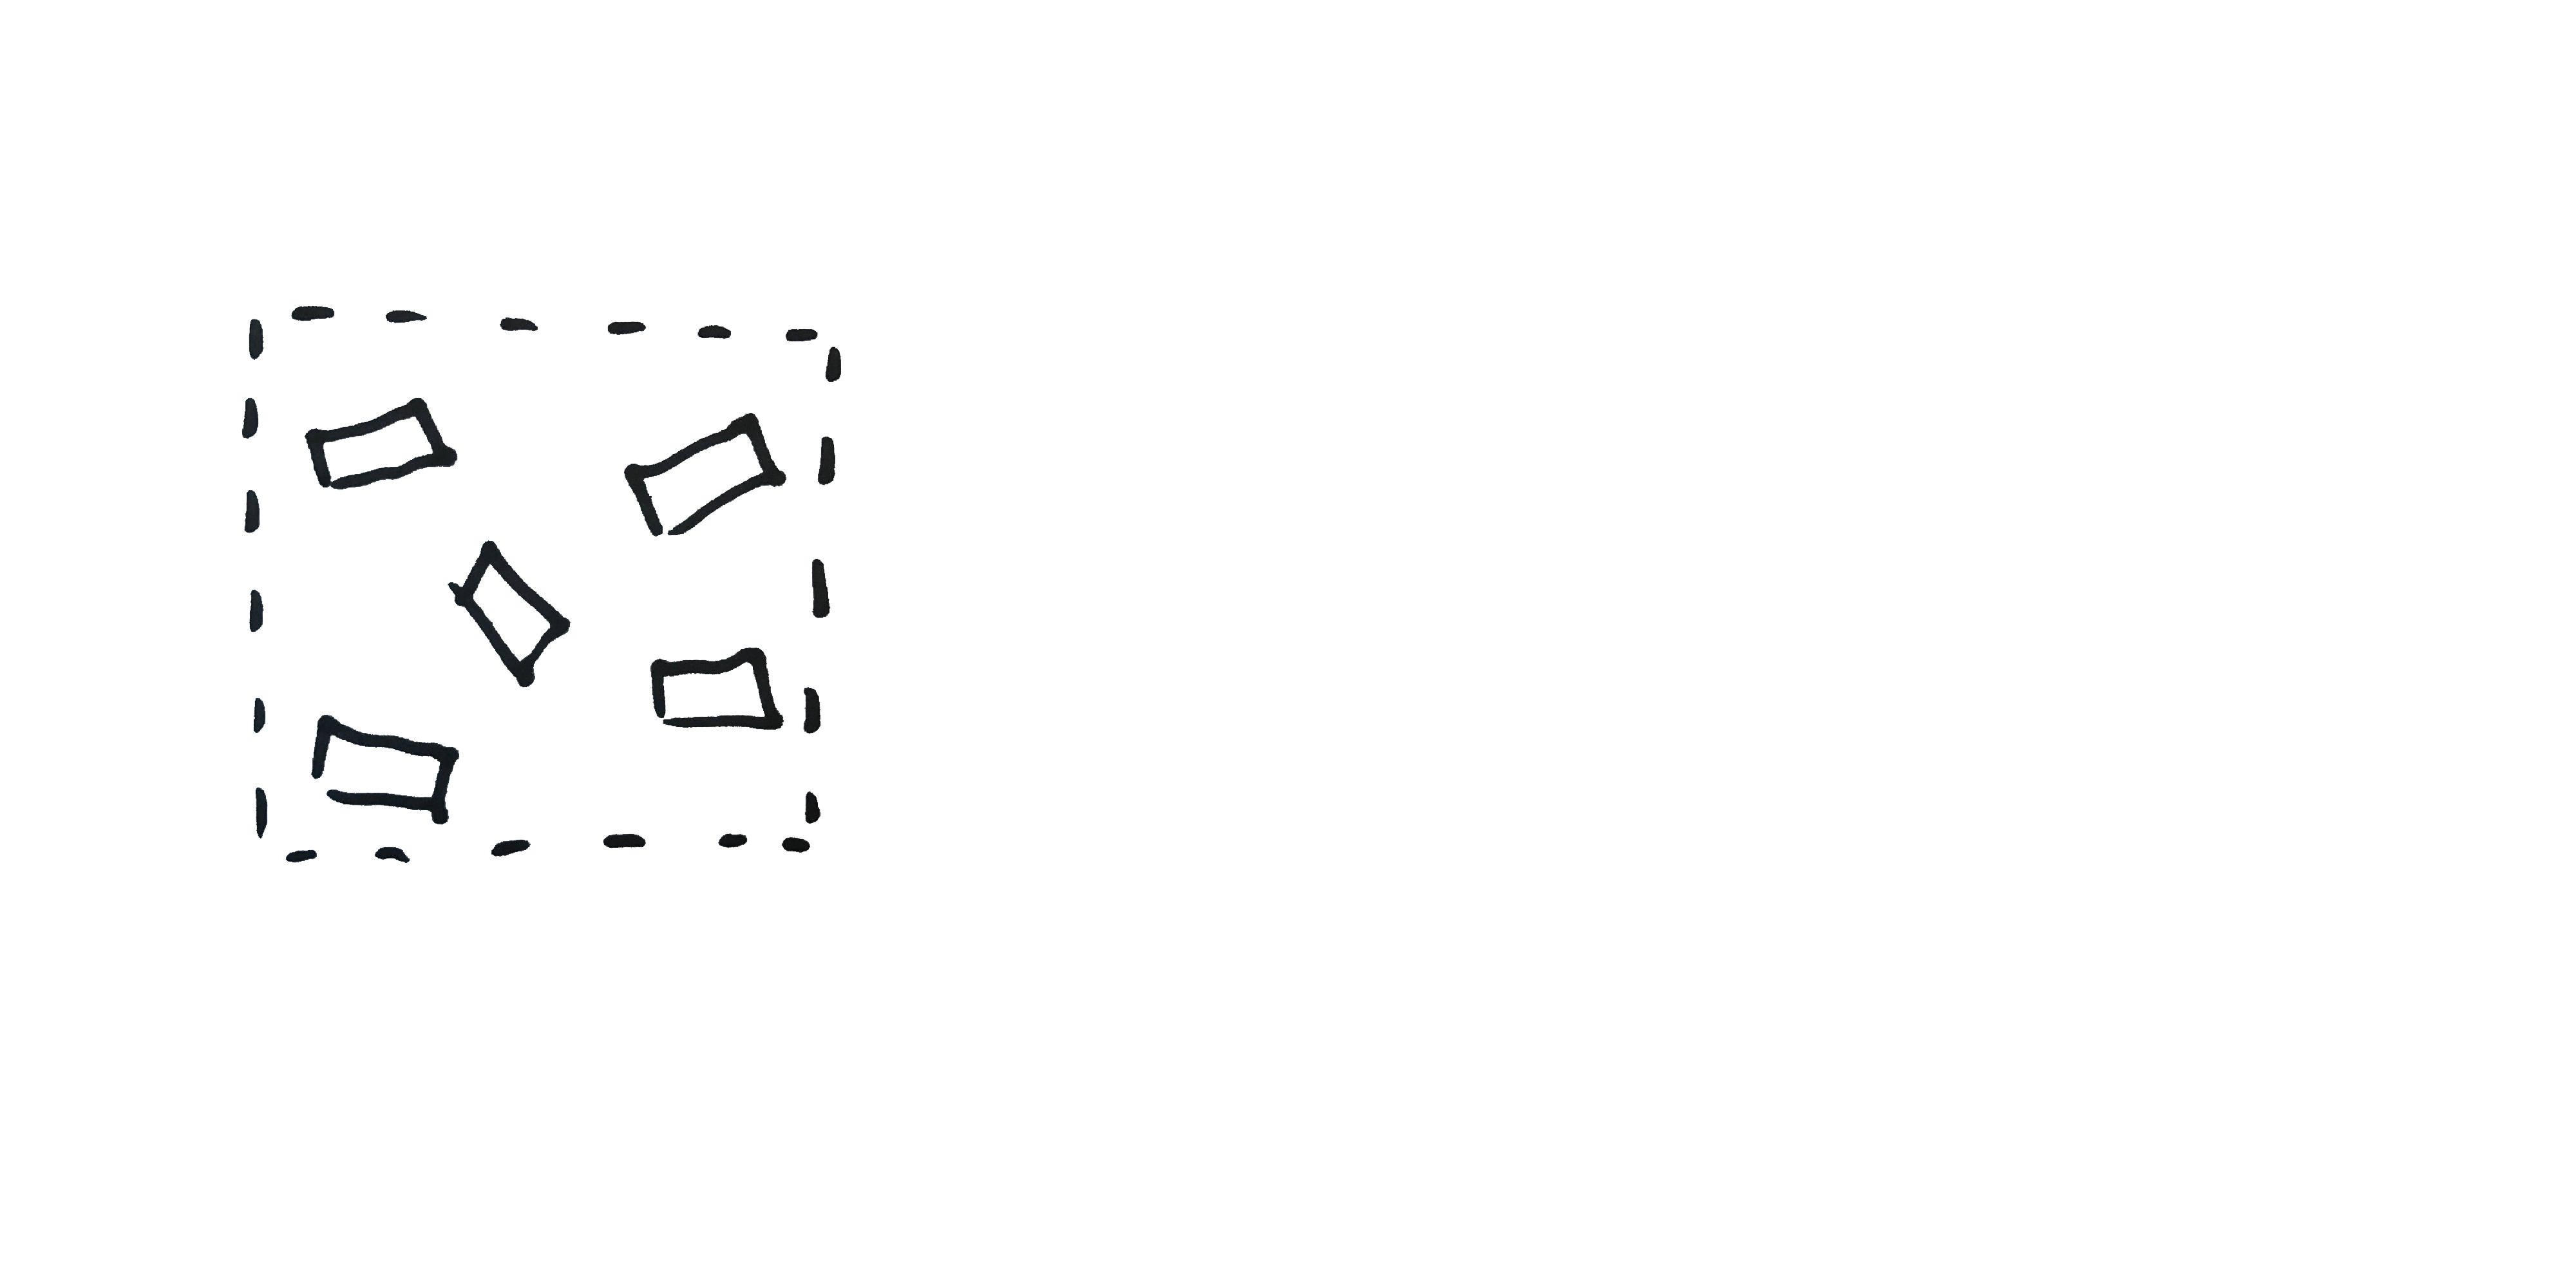
\includegraphics[height = 0.3\textheight, rotate = 180, decodearray={0.65 .8 0.84 .8 0.82 .8}]{../assets/images/block_1}};
	
	\draw[->, line width=0.5mm] (block.north east) + (-.8, -.8)-- (agent1.west);
	\draw[->, line width=0.5mm] (block.south east) + (-.8, .7)-- (agent2.west);
	
%	\draw[->, thick, color = highlight] (ledger.south east) + (-1, 1) -- (node.west);
%	\draw[->, thick, color = focus] (block1.west) + (0.5, 0) -- (client.north east);
%	\draw[->, thick, color = focus] (block1.west) + (0.5, 0) -- node[midway, xshift=7, yshift=-7] {
\includegraphics[height = 0.05\textheight, decodearray={1 1 0 1 0 1}]{../assets/images/remove}} (client.north east);
%	\draw[->, thick, color = highlight] (block2.west) + (0.5, 0) -- node[midway, xshift=7, yshift=7] {
\includegraphics[height = 0.05\textheight, decodearray={0.65 .8 0.84 .8 0.82 .8}]{../assets/images/check}} (client.south east);
	
	
\end{footnotesize}